\subsection{Drift User Interface}
\label{driftui}

To complete the implementation of the \textit{Drift} programming
environment, this section will introduce the system's visualization.
The idea for this visualization is heavily based on the concept
of \textit{immediate feedback} that was introduced in chapter \ref{bretvictor}
as well as on the original idea of a \textit{language of the system}
as introduced in chapter \ref{LanguageOfTheSystem}.

Therefor the overall goal of the system's visualization is to
give the user a bird's-eye perspective of the overall system.
This overview should show all the data dependecies that have
been built-up by the user but should also dynamically react
to either new instructions by the user but also new events in
the system itself, e.g. the finishing of a task.

Furthermore this visual representation should not replace the
original shell. It was not supposed to be a visual language
but rather a graphical representation of the data
dependencies created by the user. Using only a textual interface
like the shell, makes it \textit{easy} for the user the built-up
large structures with only a few lines of commands. This can
mislead the user into thinking that the system is still small
and managable when in reality it is a complex dependency graph
containing multiple interconnected data dependencies that
are not easy to grasp. Therefor the visual representation
is thought of as a guideline for the user, mirroring her commands
and showing their immediate effects to the overall system.
\newline

Since other workflow systems use a direct acyclic graph (DAG)
to encapsulate and represent the data dependencies as described
by the user, the first idea was to also use a DAG as a dynamic
representation of the system. Whenever the user would enter a new command,
a new vertex would appear in the DAG and whenever a task finished
the system would insert the event into the \texttt{Update} queue
that was introduced in chapter \ref{driftimplementation} and the
DAG would eliminate the corresponding vertex and update its view.

At first this was implemented in exactly that fashion. Unfortunately
this forced the decision whether vertices in the DAG represent
services and where therefor named after the name of the invoked
service, or whether vertices represent the data, being named after
the names given by the user. Although it would've been possible
to allow the user to dynamically switch between both views,
the DAG itself was discarded as a fitting visual representation.
A DAG only describes the dependency aspect of its vertices.
If there is a path from vertex $A$ to vertex $B$ then there is
a dependency between $A$ and $B$. If no such path exists, $A$
are $B$ independent of each other. That is what is captured by
the DAG.

However, the Drift language's core concepts are \textit{data}
and \textit{functionality}. Therefor both concepts exist in
the language: \textit{names} (data) and \textit{services}
(functionality). So a visual representation would need to
have two different concepts in order to represent both, names
and services.
Another important aspect of the services orchestrated by the
Drift system is their locality in terms of their inputs, outputs and
state, as was introduced in chapter
\ref{driftimplementation}. This means that no single service
invocation ever has nor needs \textit{any} global information
or global state. Its execution and its outputs only ever depend
on the data contained in its input queues and output is only
ever produced to its own output queue. As was already mentioned
in the last chapter, this is heavily reminiscent of transitions
in a Petri Net because they too only ever consume from their
input places and only ever produce to their output places.

\begin{wrapfigure}{r}{0.3\textwidth}
  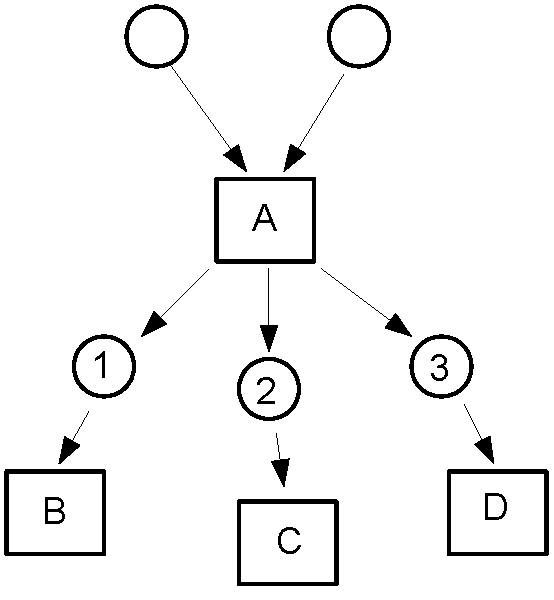
\includegraphics[scale=0.5, keepaspectratio]{pn1.pdf}
  \caption{Rough sketch example of a Petri Net.}
  \label{pn1}
\end{wrapfigure}

Interestingly, since Petri Nets too are based on two core concepts,
namely \textit{places} and \textit{transitions}, they offer different
syntax to talk about both concepts. Figure \ref{pn1} shows a very
rough sketch of the idea of a Petri Net. The Petri Net syntax
uses circles to represent places and squares to represent transitions.
Therefor Fig.\ref{pn1} shows a transition $A$ consuming from two
input places and producing to three \textit{different} output places,
$1, 2$ and $3$. These places are then also input places for the
following transactions $B, C$ and $D$ which each only depend
on their single corresponding input place.

This works perfectly fine when the Petri Net is static and modelled
without any dynamically changing parts. However, given the goal
of immediate feedback the Drift shell uses eager-evaluation and
the system is composed \textit{along the way} whenever the user
enters new commands.
Therefor it is not possible to infer or predict how many consumers
a given service invocation will have. In the worst-case scenario
all available workers will at some point consume from the
same input data source at the same time. That means that building the
system defensively one would have to add as many output places to any
service invocation as there are workers in the system.

This makes sense in the formalism and realm of Petri Nets because
here, as shown in Fig.\ref{pn1}, transition $B$ could really consume
(meaning eliminate) tokens from place $1$ but not from place $2$.
Therefor the \textit{firing} of transition $B$ is completely
independent from the firing of transition $C$ because their inputs
are different. If one would change the given model, having transition
$A$ produce to only a single output place and having transitions
$B, C$ and $D$ all consume from this single place would also
drastically change the semantics of the net. Because in that case
tokens consumed by $B$ would no longer be available to transitions
$C$ and $D$. They would naturally content for the tokens because
consuming a token is a destructable action (side effect).
\newline

However, given that the output queues in the Drift back end
are implemented using \textit{immutable} Apache Kafka queues, multiple
consumers can consume from the same queue concurrently without
any contention. Therefore, instead of modelling the
producer-consumer relationships between $A$ and $B, C$ and $D$
with different independent output places, a single output
place can be used, as shown by Fig.\ref{pn2}.

\begin{wrapfigure}{l}{0.3\textwidth}
  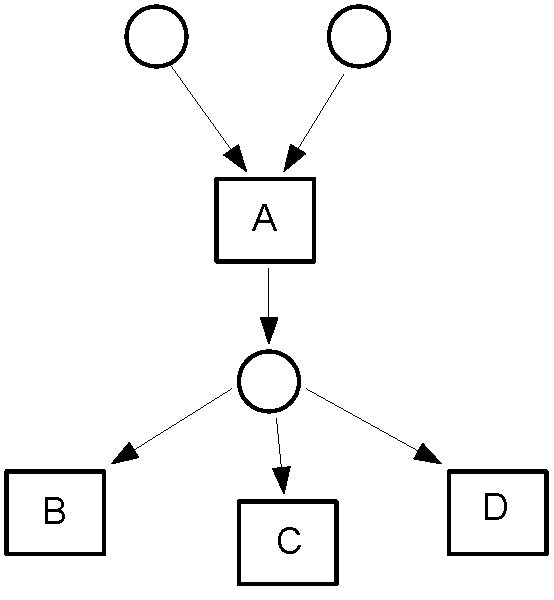
\includegraphics[scale=0.5, keepaspectratio]{pn2.pdf}
  \caption{Minimized net with \textit{different} semantics.}
  \label{pn2}
\end{wrapfigure}

It cannot be highlighted enough that using the original Petri Net
formalism the nets presented in Fig.\ref{pn1} and \ref{pn2} would
have drastically different semantics as explained earlier.
However, the Petri Net \textit{syntax} supports exactly the
same concepts as the Drift language and is therefor a better fit in terms
of visualizing a Drift system than a simple DAG, mapping names
to places and services to transitions. So \textit{only} the
\textit{visual} Petri Net syntax and not the
formalism itself is borrowed in order to visualize a drift system.

So in order implement such a visualization the browser was chosen
as a common platform that allows for ease of use and requires no
installation whatsoever, using HTML, CSS and JavaScript for
implementing the website/web interface.

Figure \ref{ui1} shows the final prototype of that user interface.
As one can see the page is split into three vertical parts. On the left
hand side there is a full Drift shell implementation in the
browser. This embedded shell works exactly like the stand alone
shell that was implemented in Java, as was presented in chapter
\ref{driftshell} and was implemented using the JavaScript
library \textit{jsTerm} \cite{jsTerm}.

In order for this shell to communicate with the Drift backend
from within the browser a small websocket server was implemented
in Java which only serves as a gateway, forwarding commands from
the shell to the back end and pushing new messages from the
\texttt{Update} queue that was presented in
chapter \ref{errormodel} to the browser using the widely known
\texttt{dot} file format to describe the new graph that should
be printed which resulted from the system update \cite{dotlang},
\cite{dotwiki}.
Since this being a full Drift shell, all the features that were
presented in chapter \ref{driftshell} are present here as well.
Only the \texttt{import} section works differently. Because
one cannot access arbitrary local files from within JavaScript
and the browser, the user needs to select to files which shall
be imported via a GUI wizard, which is the same that is used
for whenever files need to be uploaded on any other website.
User selected files can then be read by the browser and therefor
their content can be uploaded to the Drfit system.
\newline

Next to the shell there is an HTML5 canvas containing the graphical
representation of the system using the already introduced Petri Net syntax.
Since most Drift sessions start by importing some local files into the
system, the graph printed on the canvas starts out containing
only unconnected places (circles) with the given name written inside
of them.
The graph is constructed in-memory using a JavaScript library called
\textit{graphlib.js}. The layout of the constructed graph on the
canvas is automatically generated using the \textit{dagre.js}
library and the final printing of the graph onto the canvas is
done using \textit{d3.js} \cite{graphlibjs}, \cite{dagrejs},
\cite{d3js}.

Any new command by the user immediately updates the graph shown
on the canvas. Services used in the command are drawn as transitions
(squares) and connected to their input places accordingly.
If the result of the command is bound to a name, a new place is
drawn and connected to the service as its output place.

If a service has finished producing its output by sending and
\texttt{EOF} token to its output queue, the update sent to the
\texttt{Update} queue will trigger the removal of the edge
connecting the service to its output place. The same thing
happens when a service consumes an \texttt{EOF} token for one
of its input queues. It sends an event notification to the
\texttt{Update} queue which will send a new graph to the
browser missing the edge between that service and the
corresponding input place.

This means that the user can watch and observe when data has been
finally consume or produced without querying its content. Live-querying
the streamed data in the shell is still possible though.
\newline

But this liveness of the system and its graphical representation
also has its drawbacks. Imagine for example that the user entered
a lot of commands, quickly building up a large graph. Because
of the spacial limitations of the shell, some of the earlier commands
might have already been pushed out of the scope of the shell terminal.
If the user now wants to look up what command created a specific
place, she would have to scroll up, looking for the name and command
that created \textit{that} particular place.

To avoid having to do this, the graph provides a mouse-hover feature.
If the user hovers over a place, a pop-up will contain the command that
created that place. This is the graphical equivalent of the
history operators \texttt{?} and \texttt{??} that were introduced
in chapter \ref{driftlang}. Of course the mouse-hover pop-up will
contain the original command and input place names, even when
some of the original inputs have now been overwritten by newer
commands.

Another example would be, if the user entered a command and then
went for a break. Since service vertices are removed whenever
the corresponding worker finished the task execution, only
the names remain after a command was completed.
That means that the user might issue some commands, go for
a break and then come back later and find only the result
names she used. Since names are supposed to be chosen wisely, conveying
as much semantics as possible, this might be enough.
But what happens if the user \textit{does} want to revisit
how a certain name got created?

This is what the third column on the far right is for. It contains
an event time line, just like Bret Victor's time bar as introduced
in chapter \ref{bretvictor}. Whenever the user enters a new command,
the current state of the graph is snapshotted and stored in-memory
\footnote{A future implementation could feature allowing to
persist these snapshots to the local filesystem, see chapter
\ref{futurework}}.
By hovering over the different bubbles in the time line the
canvas will show the graph that was snapshotted at the time
the event was created, e.g. the time the user issued the command.
Therefor the user can ``scroll through history'' by just moving
her mouse along the time bar.

